% Make nice A4 pages for print:
%\usepackage{pgfpages}
%\pgfpagesuselayout{resize to}[a4paper,border shrink=5mm,landscape]

\beamertemplatenavigationsymbolsempty

\setbeamertemplate{bibliography item}[text]

\usepackage[type={CC},modifier={by-sa},version={4.0}]{doclicense}

\usepackage[utf8]{inputenc}
\usepackage{hyperref}
\usepackage{breakurl}
\usepackage{graphicx}
\usepackage{pgfplots}
\usepackage{pgf}
\usepackage{tikz}
\usetikzlibrary{positioning}
\usetikzlibrary{arrows}
\usetikzlibrary{decorations.markings}
\usetikzlibrary{calc}
\usetikzlibrary{matrix}
\usetikzlibrary{shapes}
\usetikzlibrary{decorations.pathmorphing}
\usetikzlibrary{fit}
\usetikzlibrary{backgrounds}
\usetikzlibrary{plotmarks}
\usepackage{stmaryrd}
\usepackage{listings}
\usepackage{pdflscape}
\usepackage{perpage}
\usepackage{appendixnumberbeamer}

%\usepackage[thmmarks,amsmath,amsthm]{ntheorem} % already included in beamer
\usepackage{thm-restate}

\usepackage[sort&compress,numbers]{natbib}  % to be have \citet, \citeauthor, \citeyear

\MakePerPage{footnote}

\tikzstyle{o}=[r,ppBlue]
\tikzstyle{r}=[thick,rectangle,align=center]
\tikzstyle{t}=[r,ppTrans] %,font=\bfseries]
\tikzstyle{dd}=[densely dashed]
\tikzstyle{n}=[r,ppBlue]
\tikzstyle{p}=[r,ppRed]
\tikzstyle{ppRed}  =[draw=red,  fill=  red!20]
\tikzstyle{ppBlue} =[draw=blue, fill= blue!20]
\tikzstyle{ppGreen}=[draw=green,fill=green!20]
\tikzstyle{ppTrans}=[draw=none, fill=none]

\usetheme{Warsaw}

\useoutertheme[subsection=true]{smoothbars}
%\useoutertheme[subsection=false]{miniframes}

\definecolor{bblue}{HTML}{D7DF01}	% yellow-ish actually, for better black/white printing
\definecolor{rred}{HTML}{C0504D}
\definecolor{ggreen}{HTML}{9BBB59}
\definecolor{ppurple}{HTML}{9F4C7C}
\definecolor{lightgray}{rgb}{0.3,0.3,0.3}
\definecolor{lightergray}{rgb}{0.9,0.9,0.9}
\definecolor{UniBlue}{RGB}{83,121,170}

\DeclareTextFontCommand\textintro{\normalfont\bfseries\itshape} % nice!
\newcommand{\intro}[2][]
{%
	\textintro{#2}%
}
\newcommand{\empha}[2][]
{%
	\emph{#2}%
}

%\theoremstyle{plain}
\newcounter{reqcounter}
\newtheorem{requirement}[reqcounter]{Requirement}

%setbeamercolor{structure}{fg=violet}

\makeatletter
\def\th@task{%
    \normalfont % body font
    \setbeamercolor{block title example}{bg=orange,fg=white}
    \setbeamercolor{block body example}{bg=orange!20,fg=black}
    \def\inserttheoremblockenv{exampleblock}
  }
\makeatother

\theoremstyle{task}
\newtheorem{task}{Task}

\newenvironment{assignment}%
{%\setbeamercolor{background canvas}{bg=violet}%
%\setbeamercolor{structure}{fg=cyan!90!black}%
 \setbeamercolor{frametitle}{bg=orange,fg=white}
\begin{frame}}%
{\end{frame}}%

\AtBeginSection[]{
  \begin{frame}
  \vfill
  \centering
  \begin{beamercolorbox}[sep=8pt,center,shadow=true,rounded=true]{title}
    \usebeamerfont{title}\insertsectionhead\par%
  \end{beamercolorbox}
  \tableofcontents
  \vfill
  \end{frame}
}




\pgfplotsset{compat=1.14}
\author{Markus Raab}


\title{L06 Strategies for Validation and Modularization}
%\date{28.04.2021}

\begin{document}


%%%%%%%%%%%%%%%%%%%%%%%%%%%%%%%%%%%%%%%%%% 
\section{Validation}
\subsection{}

\begin{frame}
	\frametitle{Learning Outcomes}
	Students will be able to
	\begin{itemize}
	\item write simple checker plugins.
	\end{itemize}
\end{frame}

\begin{frame}
	\frametitle{Checking Configurations}

	Following properties of configuration settings can be checked:

	\begin{itemize}[<+-| alert@+>]
	\item values (data types)
	\item structure
	\item constraints
	\item semantic checks (e.g., IP, folder)
	\item domain-specific checks (e.g., databases)
	\item requirements (suitable configurations)
	\item context (context-aware configurations)
	\end{itemize}
\end{frame}

\begin{frame}[allowframebreaks]
	\frametitle{}
	\elektra{} supports many other data types, each implemented in its own plugin(s):
	\begin{description}
	\item [check/type] allows us to specify CORBA data types.
	Checking ``any'' (default) is always successful.
	The record and enum types defined by CORBA are not part of this plugin but of others as explained below.

	\item [check/enum] supports a list of supported values denoted by array indexes.
	\item [check/ipaddr] checks if a string is a valid IP address.
	\item [check/path] checks presence, permissions, and type of paths in the file system.
	\item [check/date] supports to check date formats such as POSIX, ISO8601, and RFC2822.
	\item [check/range] allows us to check if numerical values are within a range.
	\item [check/validation] checks the configuration value with regular expressions.
	\item [check/condition] checks using conditionals and comparisons.
	\item [check/math] checks using mathematical expressions.
	\item [trigger/error] allows us to express unconditional failures.
	\item [check/rgbcolor] allows us to check for RGB colors.
	\item [check/macaddr] allow us to check for MAC addresses.
	\end{description}
\end{frame}

\begin{frame}[fragile]
	\frametitle{Logfile Example}

	\begin{code}[morekeywords={path},gobble=4]
	[slapd/logfile]
	  check/path:=file
	\end{code}
\end{frame}

\begin{frame}[fragile]
	\frametitle{Logfile Extensions}

	\begin{code}[morekeywords={match,path},gobble=4]
	[slapd/logfile]
	  check/path:=file
	  check/validation:=^/var/log/
	  check/validation/message:=Policy violation:
	    log files must be below /var/log
	\end{code}
\end{frame}

\begin{frame}
	\frametitle{Checking Specifications}

	The goals of checking \elektra{Spec} are:

	\begin{itemize} %[<+-| alert@+>]
	\item Defaults must be present for safe lookups.
	This goal also implies that there must be at least one valid configuration setting.
	\item Types of default values must be compatible with the types of the keys.
	\item Every contextual interpretation of a key must yield a compatible type.
	\item Links must not refer to each other in cycles.
	\item Every link and the pointee must have compatible types.
	\end{itemize}
\end{frame}

\begin{frame}[fragile]
	\frametitle{Example}

	\begin{code}[morekeywords={override},gobble=4]
	[sw/org/abc/has_true_arg]
	  type:=boolean
	  default:=0
	  override/#0:=/sw/org/abc/arg0
	  override/#1:=/sw/org/abc/arg1
	\end{code}
\end{frame}

%TODO: this part about error messages should be more relevant for H3
%  special techniques to be moved to 09.tex
\begin{frame}[fragile]
	\frametitle{Error Messages}

	Error messages are extremely important as they are the main communication channel to system administrators.\\
	Example specification:
	\vspace{1em}

	\begin{code}[morekeywords={assign,math},gobble=4]
	[a]
	  check/type:=long
	[b]
	  check/type:=long
	[c]
	  check/range:=0-10
	  assign/math:=../a+../b
	\end{code}
\end{frame}

\begin{frame}[fragile]
	\frametitle{Error Messages}

	Problems:
	\begin{itemize}[<+-| alert@+>]
	\item Generic vs.\ specific plugins
	\item General principles of good error messages~\cite{lee2011personifying}
	\item Give context
	\item Precisely locate the cause:
	\end{itemize}
	\vspace{1em}

	\pause[\thebeamerpauses]

	\begin{code}[language=CfgElektra,gobble=4]
	a=5  ; unmodified
	b=10 ; modification bit in metadata
	     ; is only set here
	c=15 ; unmodified by user but changed
	     ; later by assign/math
	\end{code}
\end{frame}

\begin{frame}[fragile]
	\frametitle{Example Error Message}
\begin{verbatim}
Sorry, I was unable to change the configuration settings!
I tried to modify b to be 10 but this caused c to be
outside of the allowed range (0-10).
\end{verbatim}
With additional verbose/debug output:
\begin{verbatim}
Module: range
At: sourcefile.c:1234
Mountpoint: /test
Configfile: /etc/testfile.conf
\end{verbatim}
\end{frame}




%%%%%%%%%%%%%%%%%%%%%%%%%%%%%%%%%%%%%%%%%% 
\section{Modularity}


\begin{frame}
	\frametitle{Types of Modularity}
	\Large
	\ExecuteMetaData[../../book/backend.tex]{definition-modularity}
\end{frame}

\subsection{Vertical}

\begin{frame}
	\frametitle{Status Quo in Free Systems}

	\begin{itemize}[<+-| alert@+>]
	\item nearly all applications use their own configuration system
	\item immense differences in configuration file formats and configuration access
	\item very high modularity
	\end{itemize}
\end{frame}

\begin{frame}
	\frametitle{Status Quo in Frameworks and Proprietary Systems}

	\begin{itemize}[<+-| alert@+>]
	\item obvious ways how to deal with configuration
	\item no differences in configuration access
	\item very low modularity
	\end{itemize}
\end{frame}

\begin{frame}[fragile]
	\frametitle{Vertical Modularity \cite{raab2016improving}}

	\intro[modularity!vertical]{Vertical modularity} is the degree of separation between different applications.
	If all applications use the same key database with a single backend or a single configuration file, applications would be coupled tightly.
	[...]

	If coupling between applications is low, for example every application uses a different configuration library or a different backend, we have a high degree of vertical modularity.
\end{frame}

\begin{frame}
	\frametitle{Retain Vertical Modularity \cite{raab2016improving}}

	\elektra{} provides two mechanisms to retain vertical modularity:

	\begin{itemize}
	\item \textbf{Mounting} configuration files facilitates different applications to use their own backend and their own configuration file.
	Furthermore, mounting enables integrating existing configuration files into the key database.
	Configuration specifications written in \elektra{Spec} allow different applications to share their configuration files with each other in a controlled way.

	%TODO: Duplicate
	\item Having frontends that implement existing \textbf{APIs} decouple applications from each other.
	These applications continue to use their specific configuration accesses, but \elektra{} redirects their configuration accesses to the shared key database.
	\end{itemize}
\end{frame}

\begin{frame}[fragile]
	\frametitle{Vertical Modularity \cite{raab2016improving}}
	Mountpoints can also be a part of the specification:

	\begin{code}[language=Cpp,gobble=4,showspaces=no]
	[ntp]
	  mountpoint:=ntp.conf
	[sw/libreoffice]
	  mountpoint:=libreoffice.conf
	\end{code}

	\begin{task}
	Which type of specification is this?
	\end{task}
\end{frame}

\begin{frame}
	\frametitle{Types of Specifications}
	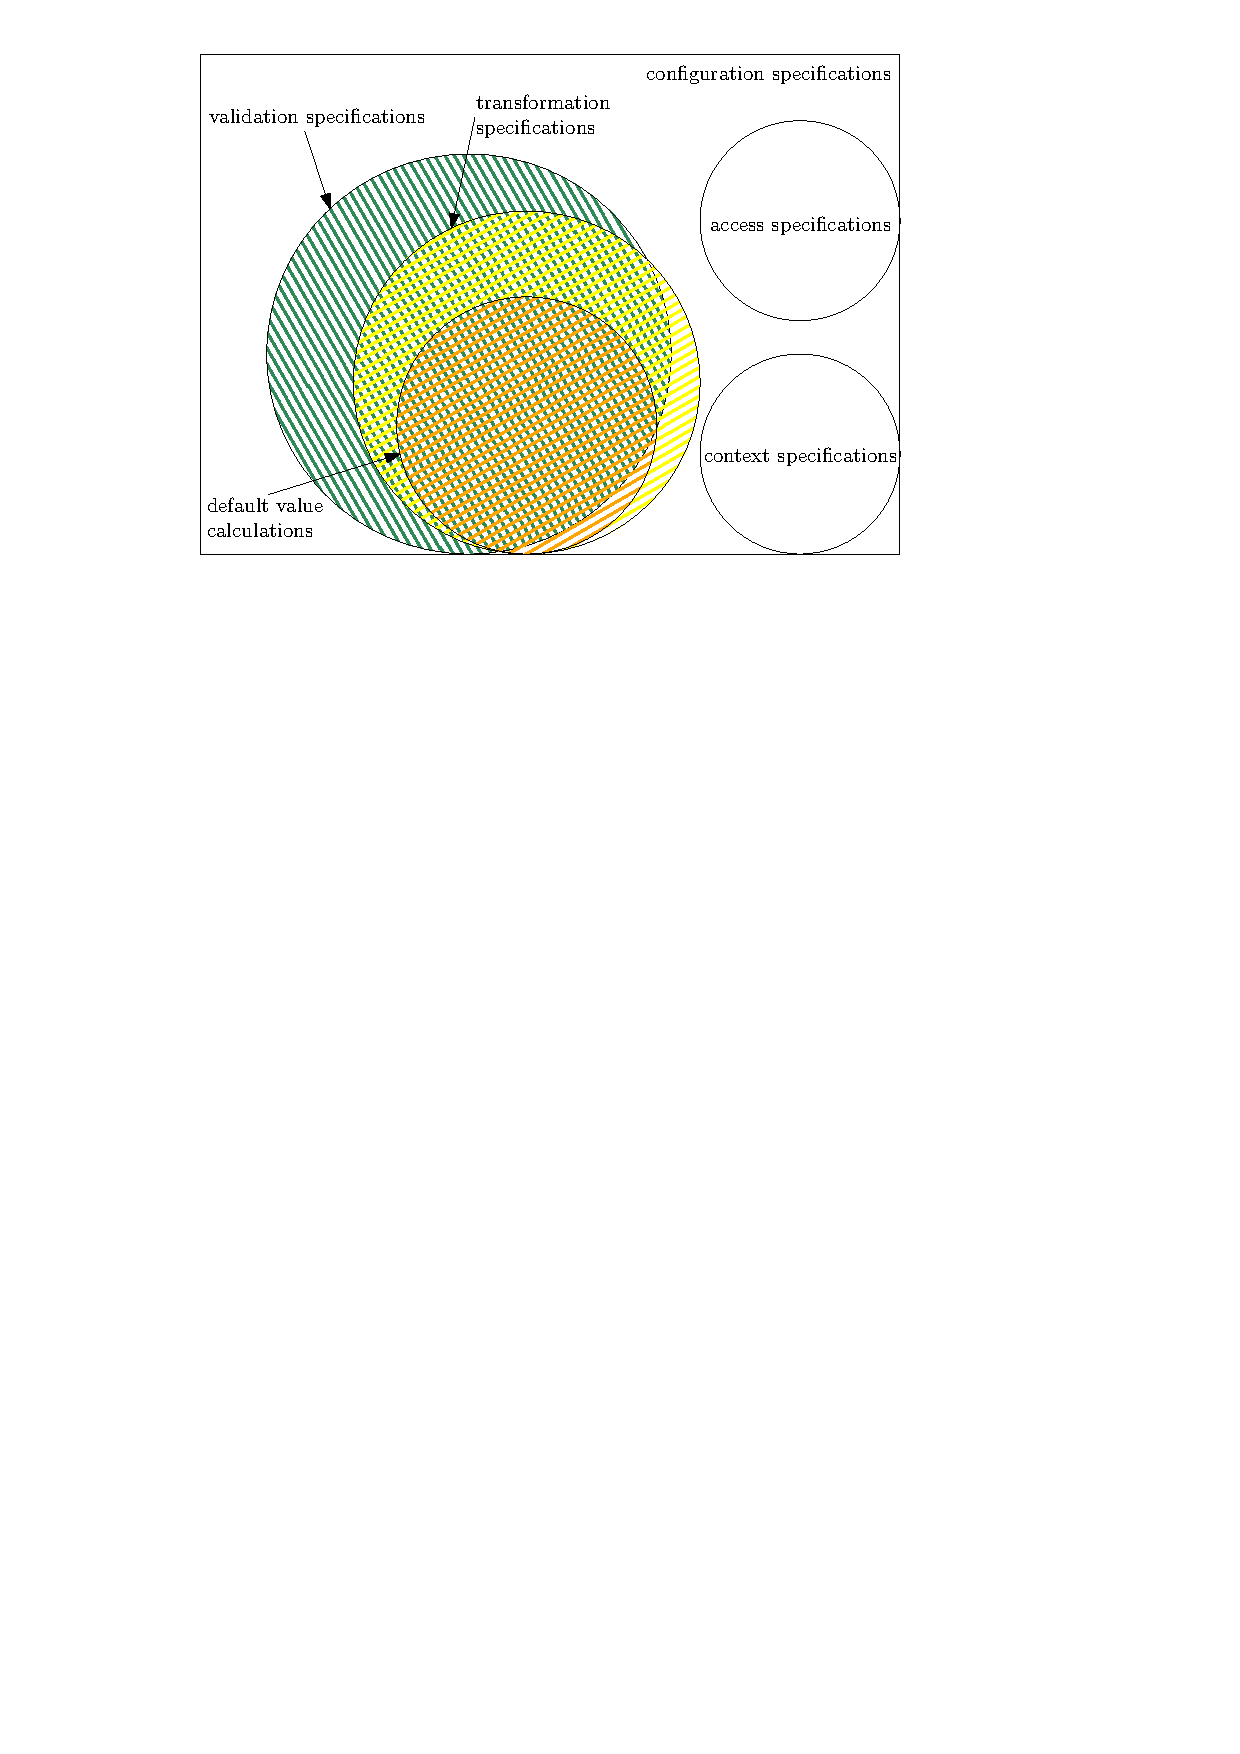
\includegraphics[scale=0.8]{specifications}
\end{frame}

\begin{frame}
	\frametitle{Vertical Modularity}
	\begin{columns}[c]
	\column{7cm}
	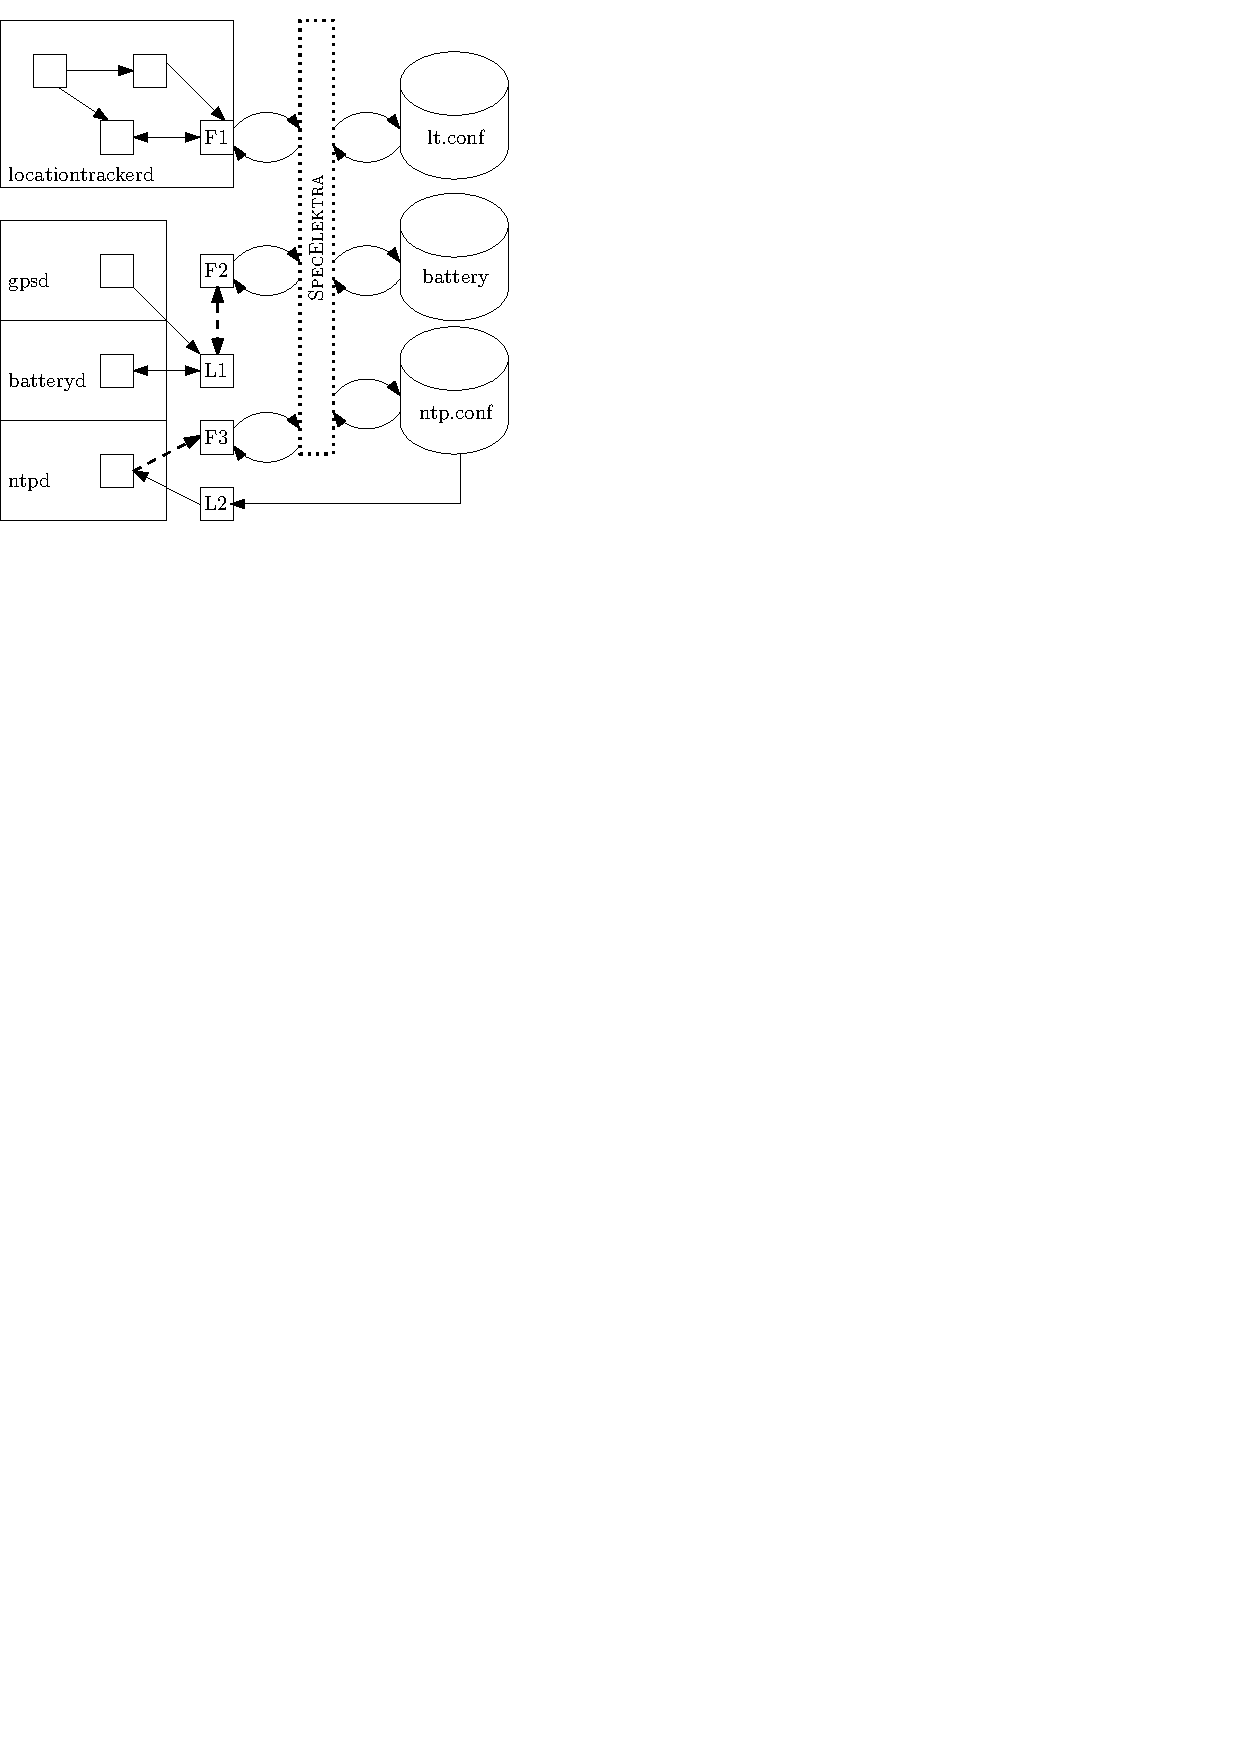
\includegraphics[scale=0.75]{verticalmodularity}
	\column{4cm}
	Needed to keep applications independently.

	Boxes are applications, cylinders are configuration files, F? are frontends or frontend adapters, L? are configuration libraries~\cite{raab2016improving}.
	\end{columns}
\end{frame}



\subsection{Horizontal}

\begin{frame}
	\frametitle{Horizontal Modularity \cite{raab2016improving}}

	\intro[Modularity!horizontal]{Horizontal modularity} is ``the degree of separation in configuration access code''~\cite{raab2016improving}. 
	A higher degree of horizontal modularity allows us to better separate configuration access code and plug the code together as needed.
\end{frame}

\begin{frame}
	\frametitle{Horizontal Modularity}
	\begin{columns}[c]
	\column{7cm}
	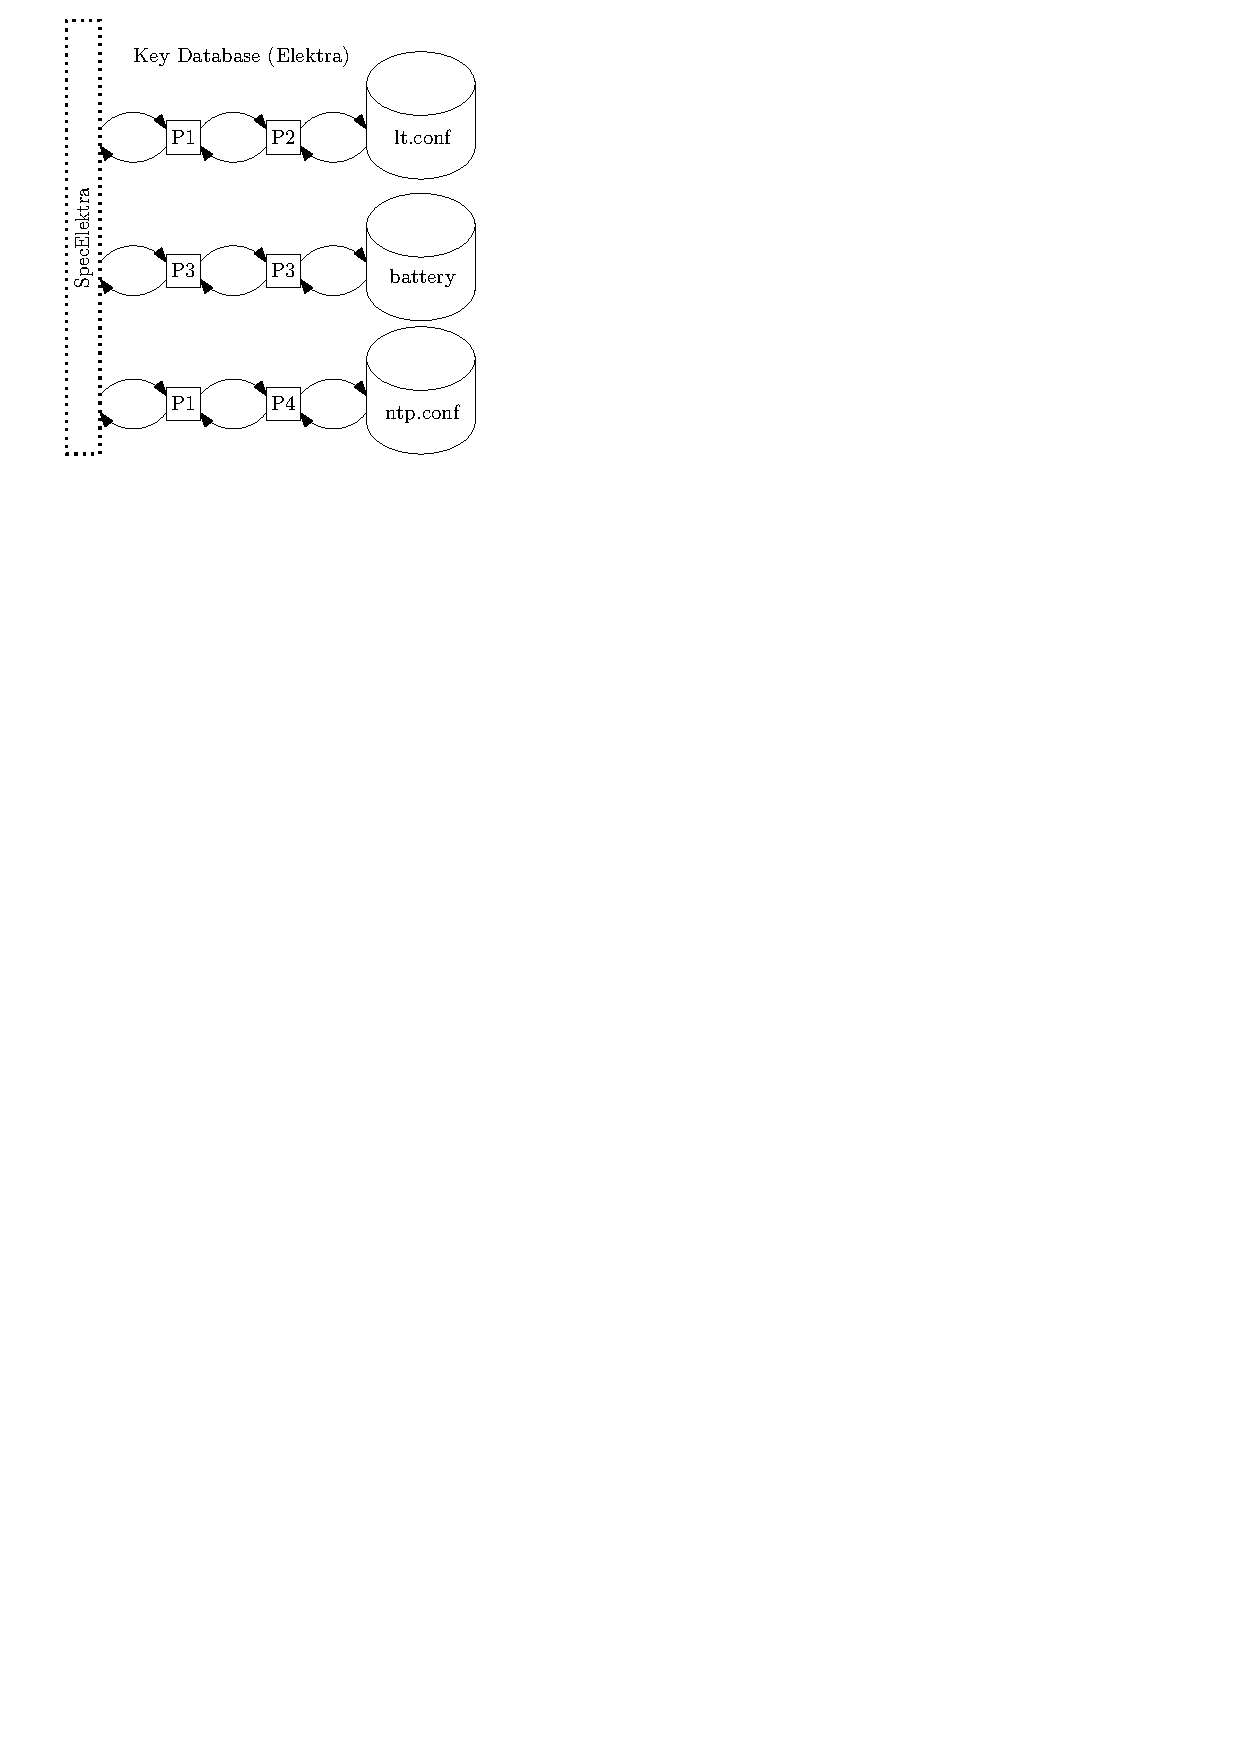
\includegraphics[scale=0.95]{horizontalmodularity}
	\column{4cm}
	Needed for validation, auto-detection, \dots \\[1cm]

	Cylinders are configuration files, P? are plugins~\cite{raab2016improving}
	\end{columns}
\end{frame}




%%%%%%%%%%%%%%%%%%%%%%%%%%%%%%%%%%%%%%%%%% 
\section{Plugins}

\subsection{Why?}


\begin{frame}
	\frametitle{Why?}
	\begin{finding}
	\methodQuestion{}
	Most developers have concerns adding dependences for more validation~(\p{84}).
	\end{finding}

	\begin{restatable}{requirement}{reqDependences}
	\label{req:dependences}
	Dependences exclusively needed to validate configuration settings must be avoided.
	\end{restatable}
\end{frame}

\begin{frame}
	\frametitle{Further Requirements}
	\begin{itemize}[<+->]
	\item \textbf{Modularity:} diverse and conflicting requirements between applications.
	Especially in validation, for example, \linebreak
	constraint solvers vs. type systems.
	\item \textbf{System-level:} specification must be enforced. Examples:
	\begin{itemize}[<+-| alert@+>]
	\item which desktop is the application started in?
	\item how many CPUs does the system have?
	\item is the filesystem local?
	\end{itemize}
	\end{itemize}
\end{frame}

\subsection{How?}

\begin{frame}
	\Large
	\ExecuteMetaData[../../book/approach.tex]{definition-plugins}
\end{frame}

\begin{frame}
	\frametitle{KeySet}

	The common data structure between plugins:
	\vspace{1cm}

	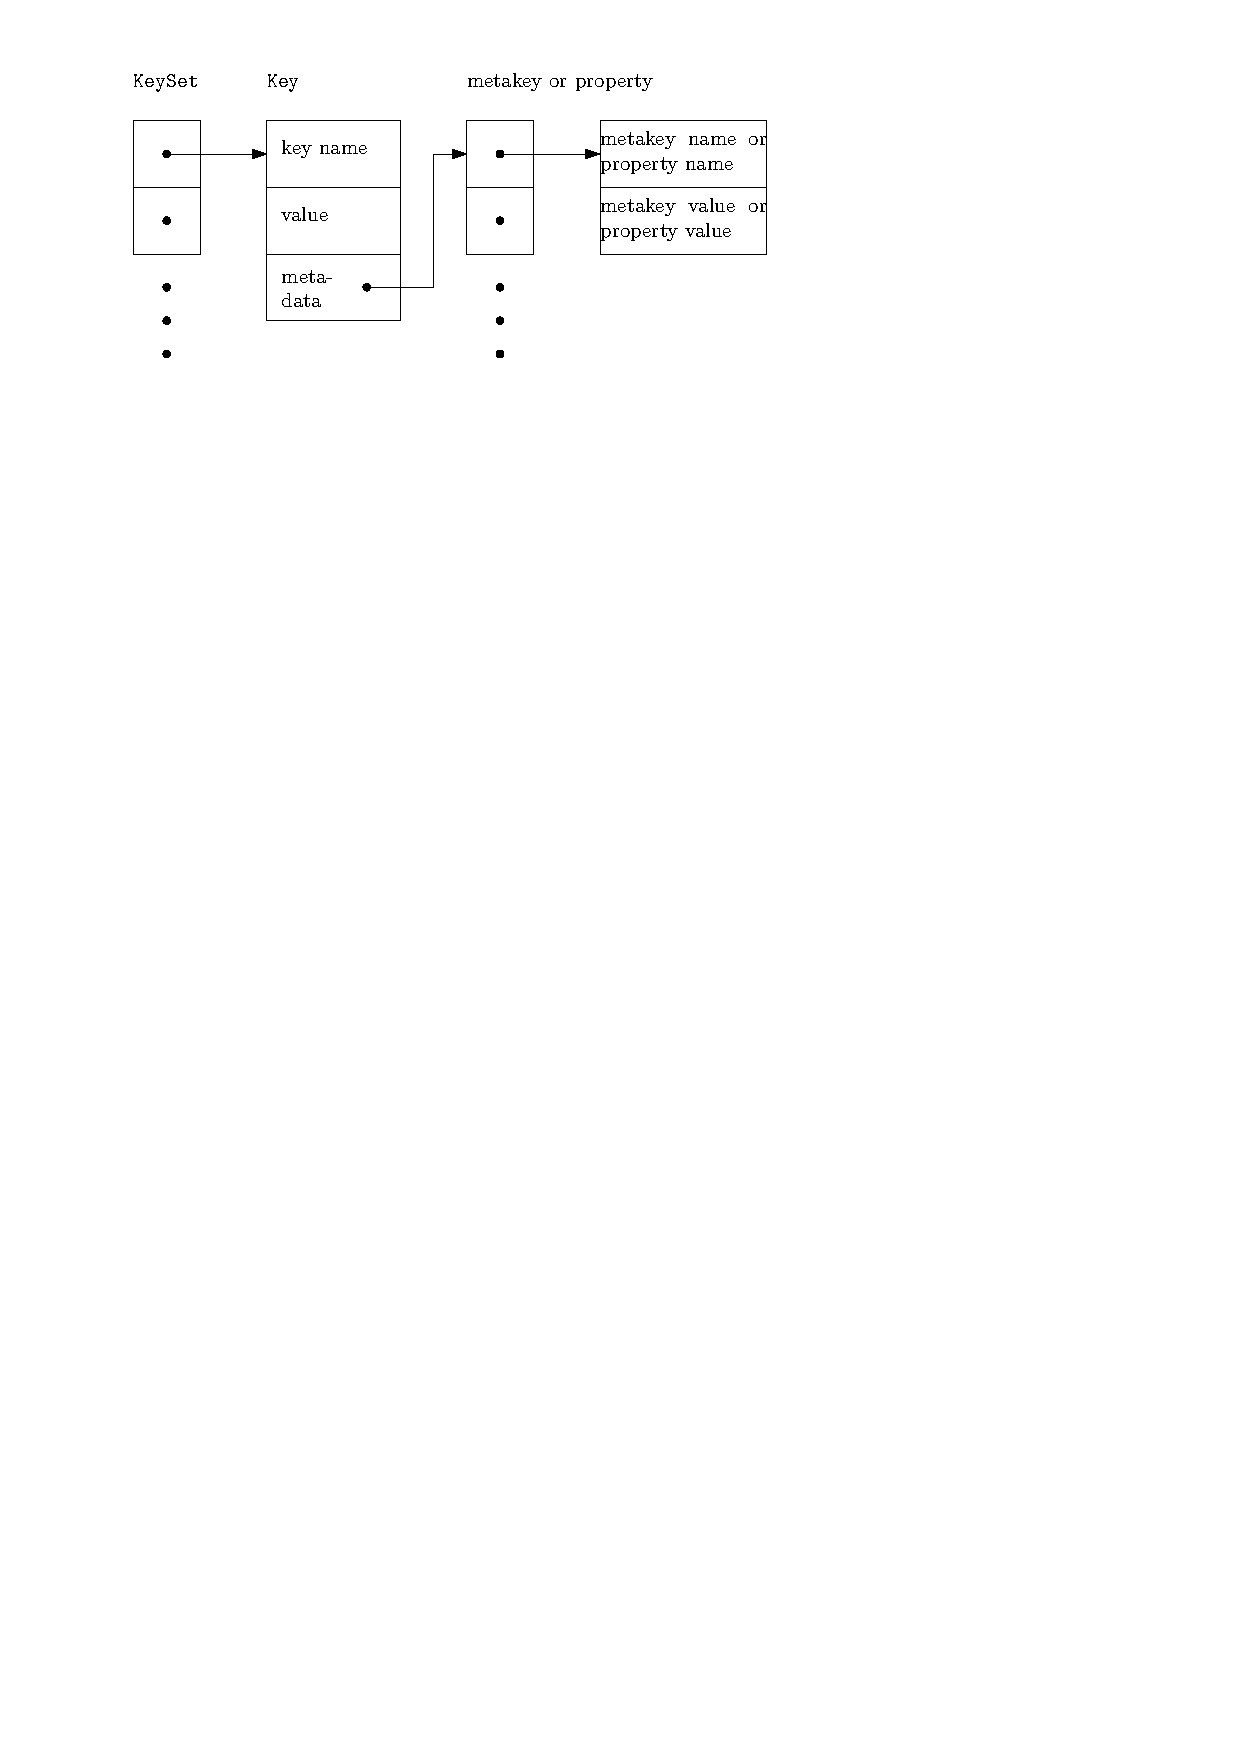
\includegraphics{keyset}
\end{frame}

\begin{frame}
	\frametitle{Metadata}

	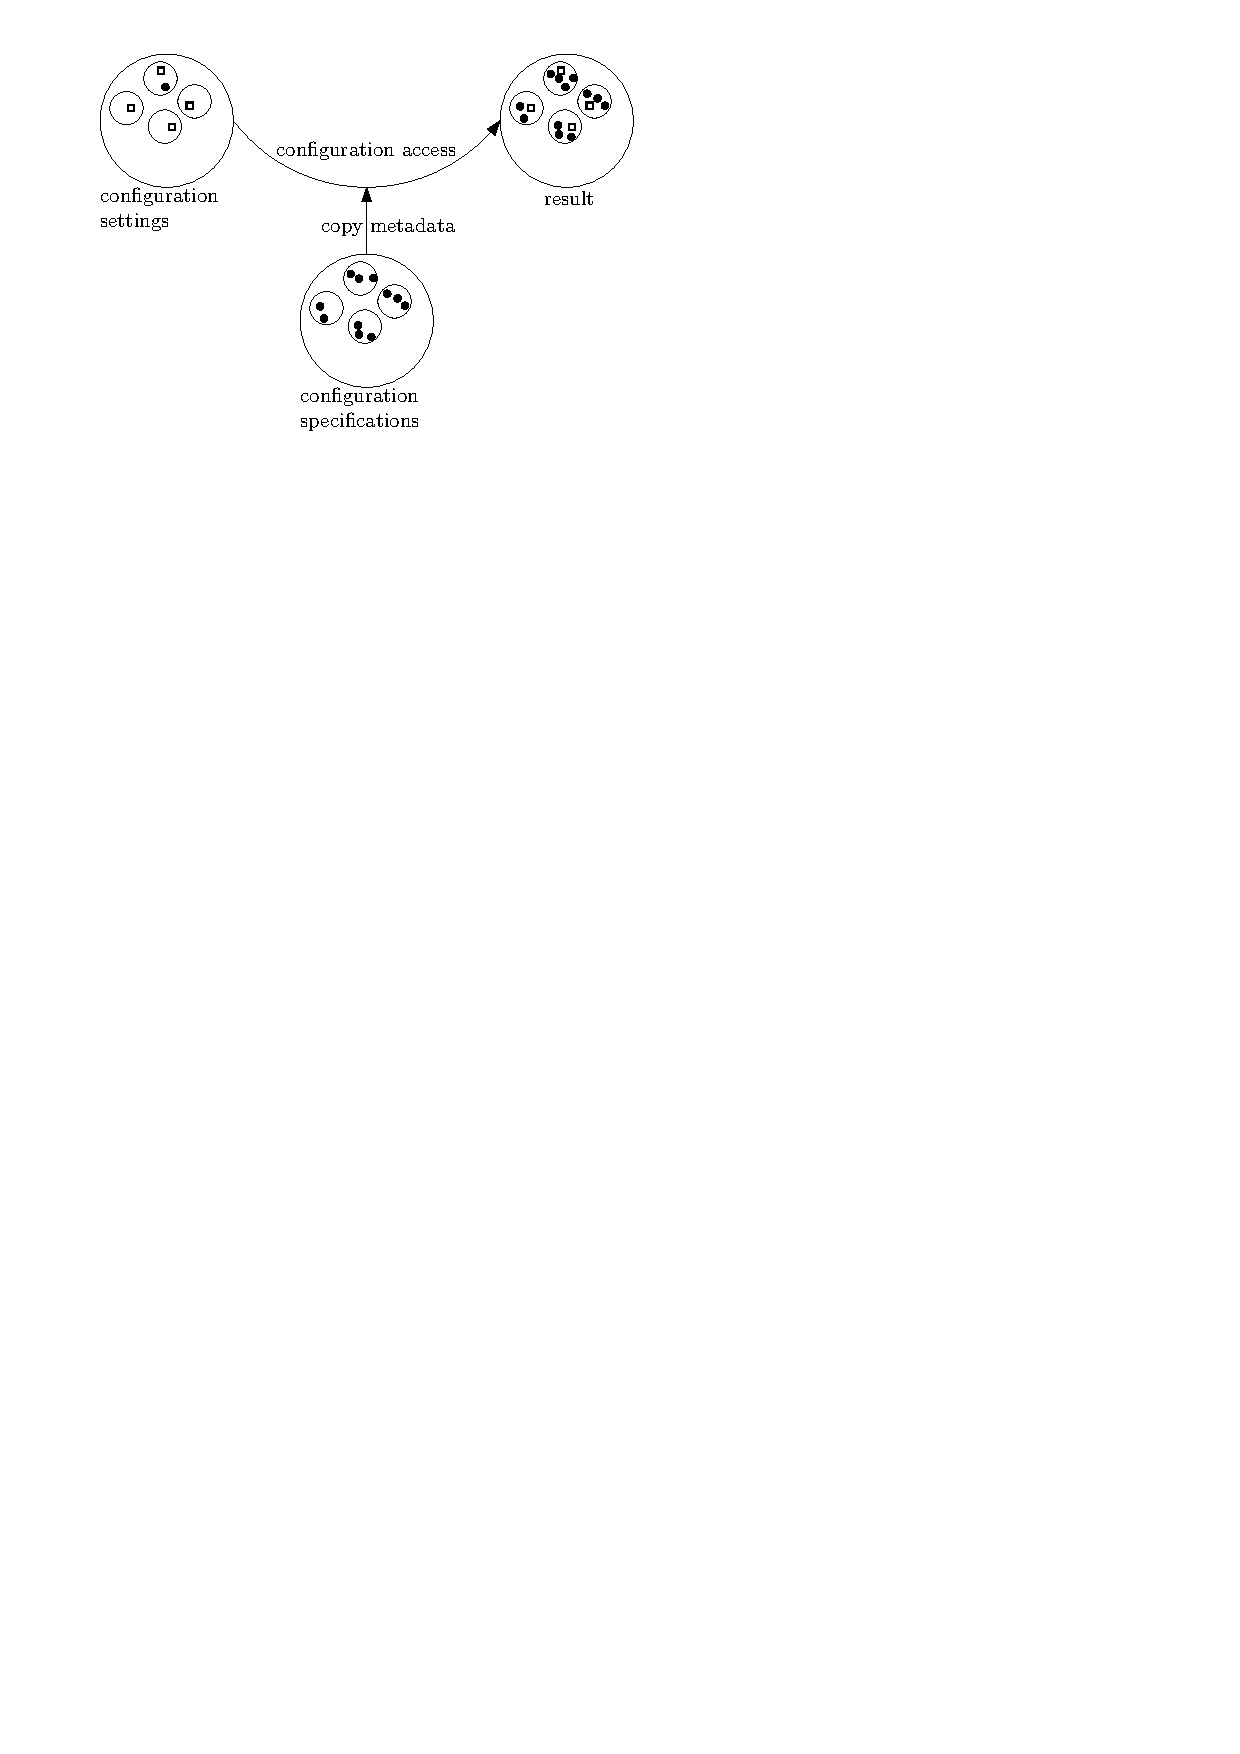
\includegraphics{metadata}
\end{frame}

\begin{frame}[fragile]
	\frametitle{Plugin Assembly}

	automatic assembling of plugins:

	\begin{itemize}[<+->]
	\item iterate over the specification and collect all key words
	\item iterate over all plugins and check if they offer key words
	\item check contract between plugins and specification
	\item of the remaining plugins: use best suited or rated
	\end{itemize}

	\vspace{1cm}

	\pause[\thebeamerpauses]

	(implemented in ^kdb mount^ / ^kdb spec-mount^ in Elektra)
\end{frame}

\begin{frame}
	SpecElektra is a dependency injection mechanism:

	\begin{itemize}[<+->]
	\item By extending the specification, new plugins are being injected into the system.
	\item The \empha{provider} abstractions in the dependences between the plugins abstract over concrete implementations of configuration access code.
	\end{itemize}
\end{frame}

\begin{frame}[fragile]
	\frametitle{Examples}
	resolve names of configuration files
	\vspace{0.3cm}

	\begin{code}[language=Cpp,gobble=4,showspaces=no]
	[example]
	  mountpoint:=/example.ini
	\end{code}
	\vspace{1cm}

	depending on operating system, e.g. UNIX:
	\vspace{0.3cm}
	\centering
	\begin{tabular}{|c|c|} \hline
	namespace & resolved path \\ \hline
	^spec^ & ^/example.ini^ \\ \hline
	^dir^ & ^${PWD}/example.ini^ \\ \hline
	^user^ & ^${HOME}/example.ini^ \\ \hline
	^system^ & ^/example.ini^ \\ \hline
	\end{tabular}
\end{frame}


%%%%%%%%%%%%%%%%%%%%%%%%%%%%%%%%%%%%%%%%%%
\section{Meeting}

%\subsection{Recapitulation}
%
%\begin{frame}
%	\frametitle{Definition}
%
%	\intro[configuration management tool]{Configuration Management Tools}:
%
%	\pause
%
%	\begin{itemize}
%	\item help people involved in configuration management.
%	\item have means to describe the desired configuration of the whole managed system.
%	\item try to converge the actual configuration to the desired one~\cite{burgess1995cfengine}.
%	\end{itemize}
%\end{frame}
%
%\begin{frame}
%	\frametitle{Possible Benefits of CM}
%
%	\pause
%
%	\begin{itemize} % [<+-| alert@+>]
%	\item All advantages scripts have: \\
%		Documentation, Customization, Reproducability
%	\item Declarative description of the system \\
%		(Infrastructure as Code~\cite{waldemar2013testing})
%	\item Less configuration drift
%	\item Error handling
%	\item Pull/Push
%	\item Reusability
%	\item (Resource) Abstractions
%	\end{itemize}
%\end{frame}
%
%\begin{frame}
%	\frametitle{CM Languages}
%
%	\begin{itemize}[<+-| alert@+>]
%	\item What is the relationship to software configuration management (Proteus/PCL)?
%	\item[] Build systems may provide configuration management features.
%	\item How is it possible to provide referential transparency both for the configuration specification language and for the system itself (NIX, GNU Guix)?
%	\item[] By functional languages and file system (layouts).
%	\item Which notations for CM exist?
%	\item[] Text,  Graphical (UML), Semi-structured, Key-value, Structured
%	\end{itemize}
%\end{frame}
%
%\begin{assignment}
%	\begin{task}
%	Break.
%	\end{task}
%\end{assignment}
%
%\begin{frame}
%	\frametitle{Checking Configurations vs. Specifications}
%
%	\pause
%
%	E.g. following properties of configuration settings can be checked:
%
%	\begin{itemize}
%	\item values (data types)
%	\item structure
%	\item constraints
%	\item semantic checks (e.g., IP, folder)
%	\item domain-specific checks (e.g., databases)
%	\end{itemize}
%
%	\vspace{1em}
%	E.g. following properties of configuration specifications can be checked:
%
%	\begin{itemize}
%	\item Types of default values must be compatible with the types of the keys.
%	\item Defaults must be present for safe lookups.
%	\end{itemize}
%\end{frame}
%
%\begin{frame}[fragile]
%	\frametitle{Error Messages}
%
%	Problems:
%	\begin{itemize} %[<+-| alert@+>]
%	\item Generic vs.\ specific plugins
%	\item General principles of good error messages~\cite{lee2011personifying}
%	\item Give context
%	\item Precisely locate the cause
%	\end{itemize}
%\end{frame}
%
%\begin{frame}
%	\frametitle{Types of Modularity}
%	\Large
%	\ExecuteMetaData[../../book/backend.tex]{definition-modularity}
%\end{frame}
%
%\begin{frame}
%	\frametitle{Metadata}
%
%	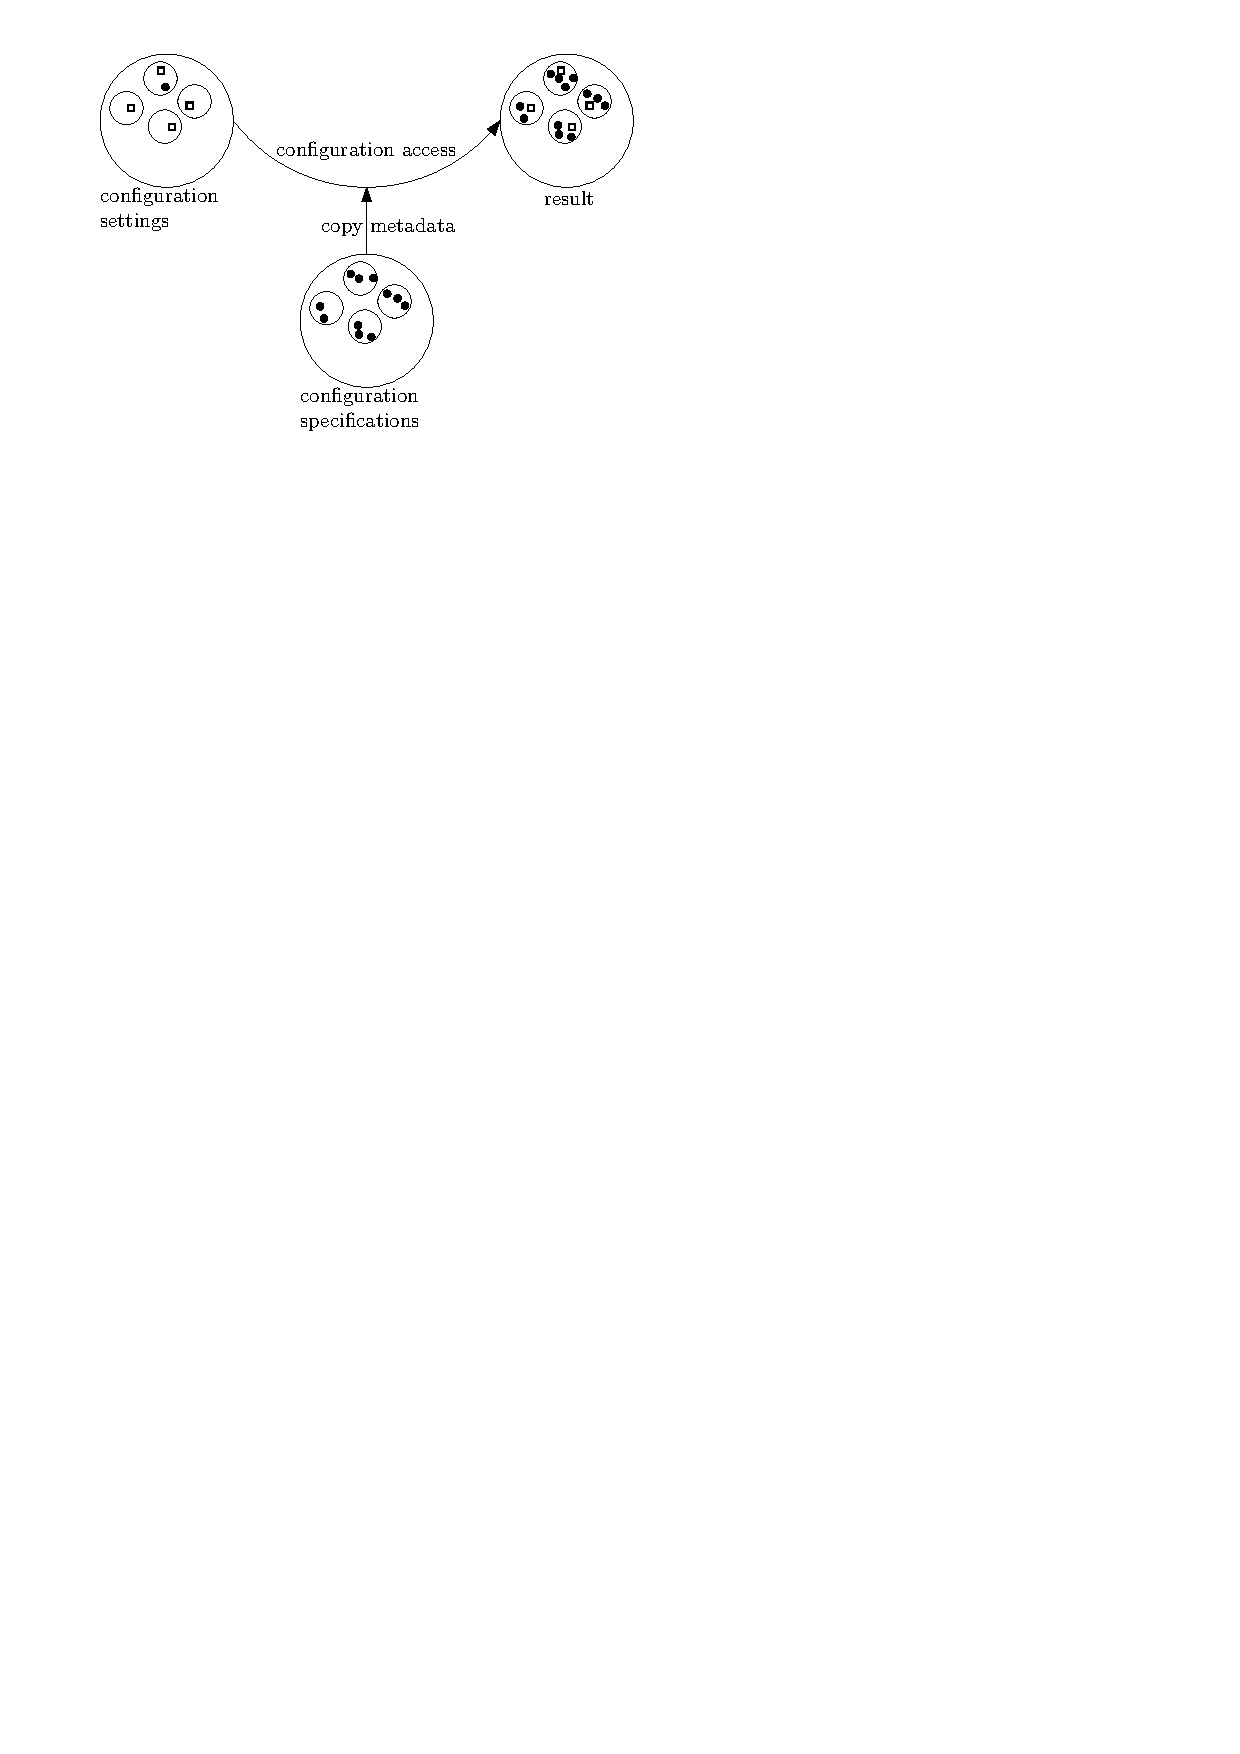
\includegraphics{metadata}
%\end{frame}
%
%\begin{assignment}
%	\begin{task}
%	Break.
%	\end{task}
%\end{assignment}
%
%\subsection{Assignments}
%
%\begin{assignment}
%	Please add slides for talk in TUWEL \textbf{and} private git repo, dates:
%
%	\begin{itemize}[<+-| alert@+>]
%	\item 12 May: submission slides
%	\item 26 May: peer review 
%	\end{itemize}
%\end{assignment}
%
%\begin{assignment}
%	Task for H3?
%\end{assignment}
%
%\begin{assignment}
%	Updated Ansible Link: \url{https://galaxy.ansible.com/elektra_initiative/libelektra}
%\end{assignment}
%
%\subsection{Preview}
%
%\begin{frame}
%	\frametitle{Outlook}
%
%	\begin{itemize} %[<+-| alert@+>]
%	\item Terms and Properties
%	\item Pitfalls
%	\item Unused Settings
%	\end{itemize}
%\end{frame}
%


\appendix

\begin{frame}[allowframebreaks]
	\bibliographystyle{plainnat}
	\bibliography{../shared/elektra.bib}
\end{frame}



\end{document}
